\documentclass{article}
\usepackage{graphicx}
\usepackage{makecell}
\usepackage[T1]{fontenc}
%\usepackage{tgpagella}      
\usepackage[dvipsnames]{xcolor}
\usepackage{booktabs}
\usepackage{comment}
\usepackage{longtable}
\usepackage{tgpagella} 
\usepackage{xfrac} 
\usepackage{float} 
\usepackage{colortbl}
\usepackage{hyperref}
%\RequirePackage{fontawesome}

\hypersetup{
    colorlinks=true, 
    linktoc=all,     
    linkcolor=black!80,
}
\renewcommand{\arraystretch}{1.4}
\newcommand{\must}{\cellcolor{Green}{M}}
\newcommand{\should}{\cellcolor{LimeGreen}{S}}
\newcommand{\could}{\cellcolor{RedOrange}{C}}
\newcommand{\wont}{\cellcolor{BrickRed}{W}}

\title{\huge Documentazione}
\author{Gabriele Chignoli}
\date{Maggio 2025}
\begin{document}
\maketitle
\newpage
\tableofcontents
\newpage

\section{Gestione del Progetto}
\subsection{Ciclo di Vita del Software}
Dopo un'analisi dei principali modelli disponibili per la modellazione del ciclo di vita del software, si è giunti alla conclusione che sia gli approcci "pesanti" che quelli più agili hanno utili proprietà che vanno combinate per portare ad un processo più, secondo il team, completo e "umano".  \newline 

Dei processi pesanti, viene considerata la pianificazione iniziale fondamentale, per garantire che il progetto segua nel lungo termine dei binari definiti entro cui operare. Tuttavia, si considera che tale processo rischi di diventare troppo morboso, e l'impossibilità di tornare ad operare su fasi iniziali già completate, viene vista come una grande limitazione. 

Per questi motivi è stato deciso di adottare il \textbf{Modello a Cascata} come modello base per la produzione del progetto; di questo, si intende poter "risalire la cascata" ogni qualvolta sia necessario (credendo nel fatto che le risalite diminuiscano con l'avanzamento del progetto), risultando così in parte simile ad un approccio evolutivo, senza tuttavia l'obbligo di eseguire tutte le fasi ad ogni ciclo. Infine, si considerano le tre fasi finali di implementazione, testing e manutenzione come un processo continuo in cui ogni parte è fondamentale per la seguente, e necessita di quella che l'ha preceduta. \newline 

Tenendo in mente queste accortezze, si è tentato di rappresentare anche graficamente il modello adottato:

\begin{figure}[H]
    \centering
    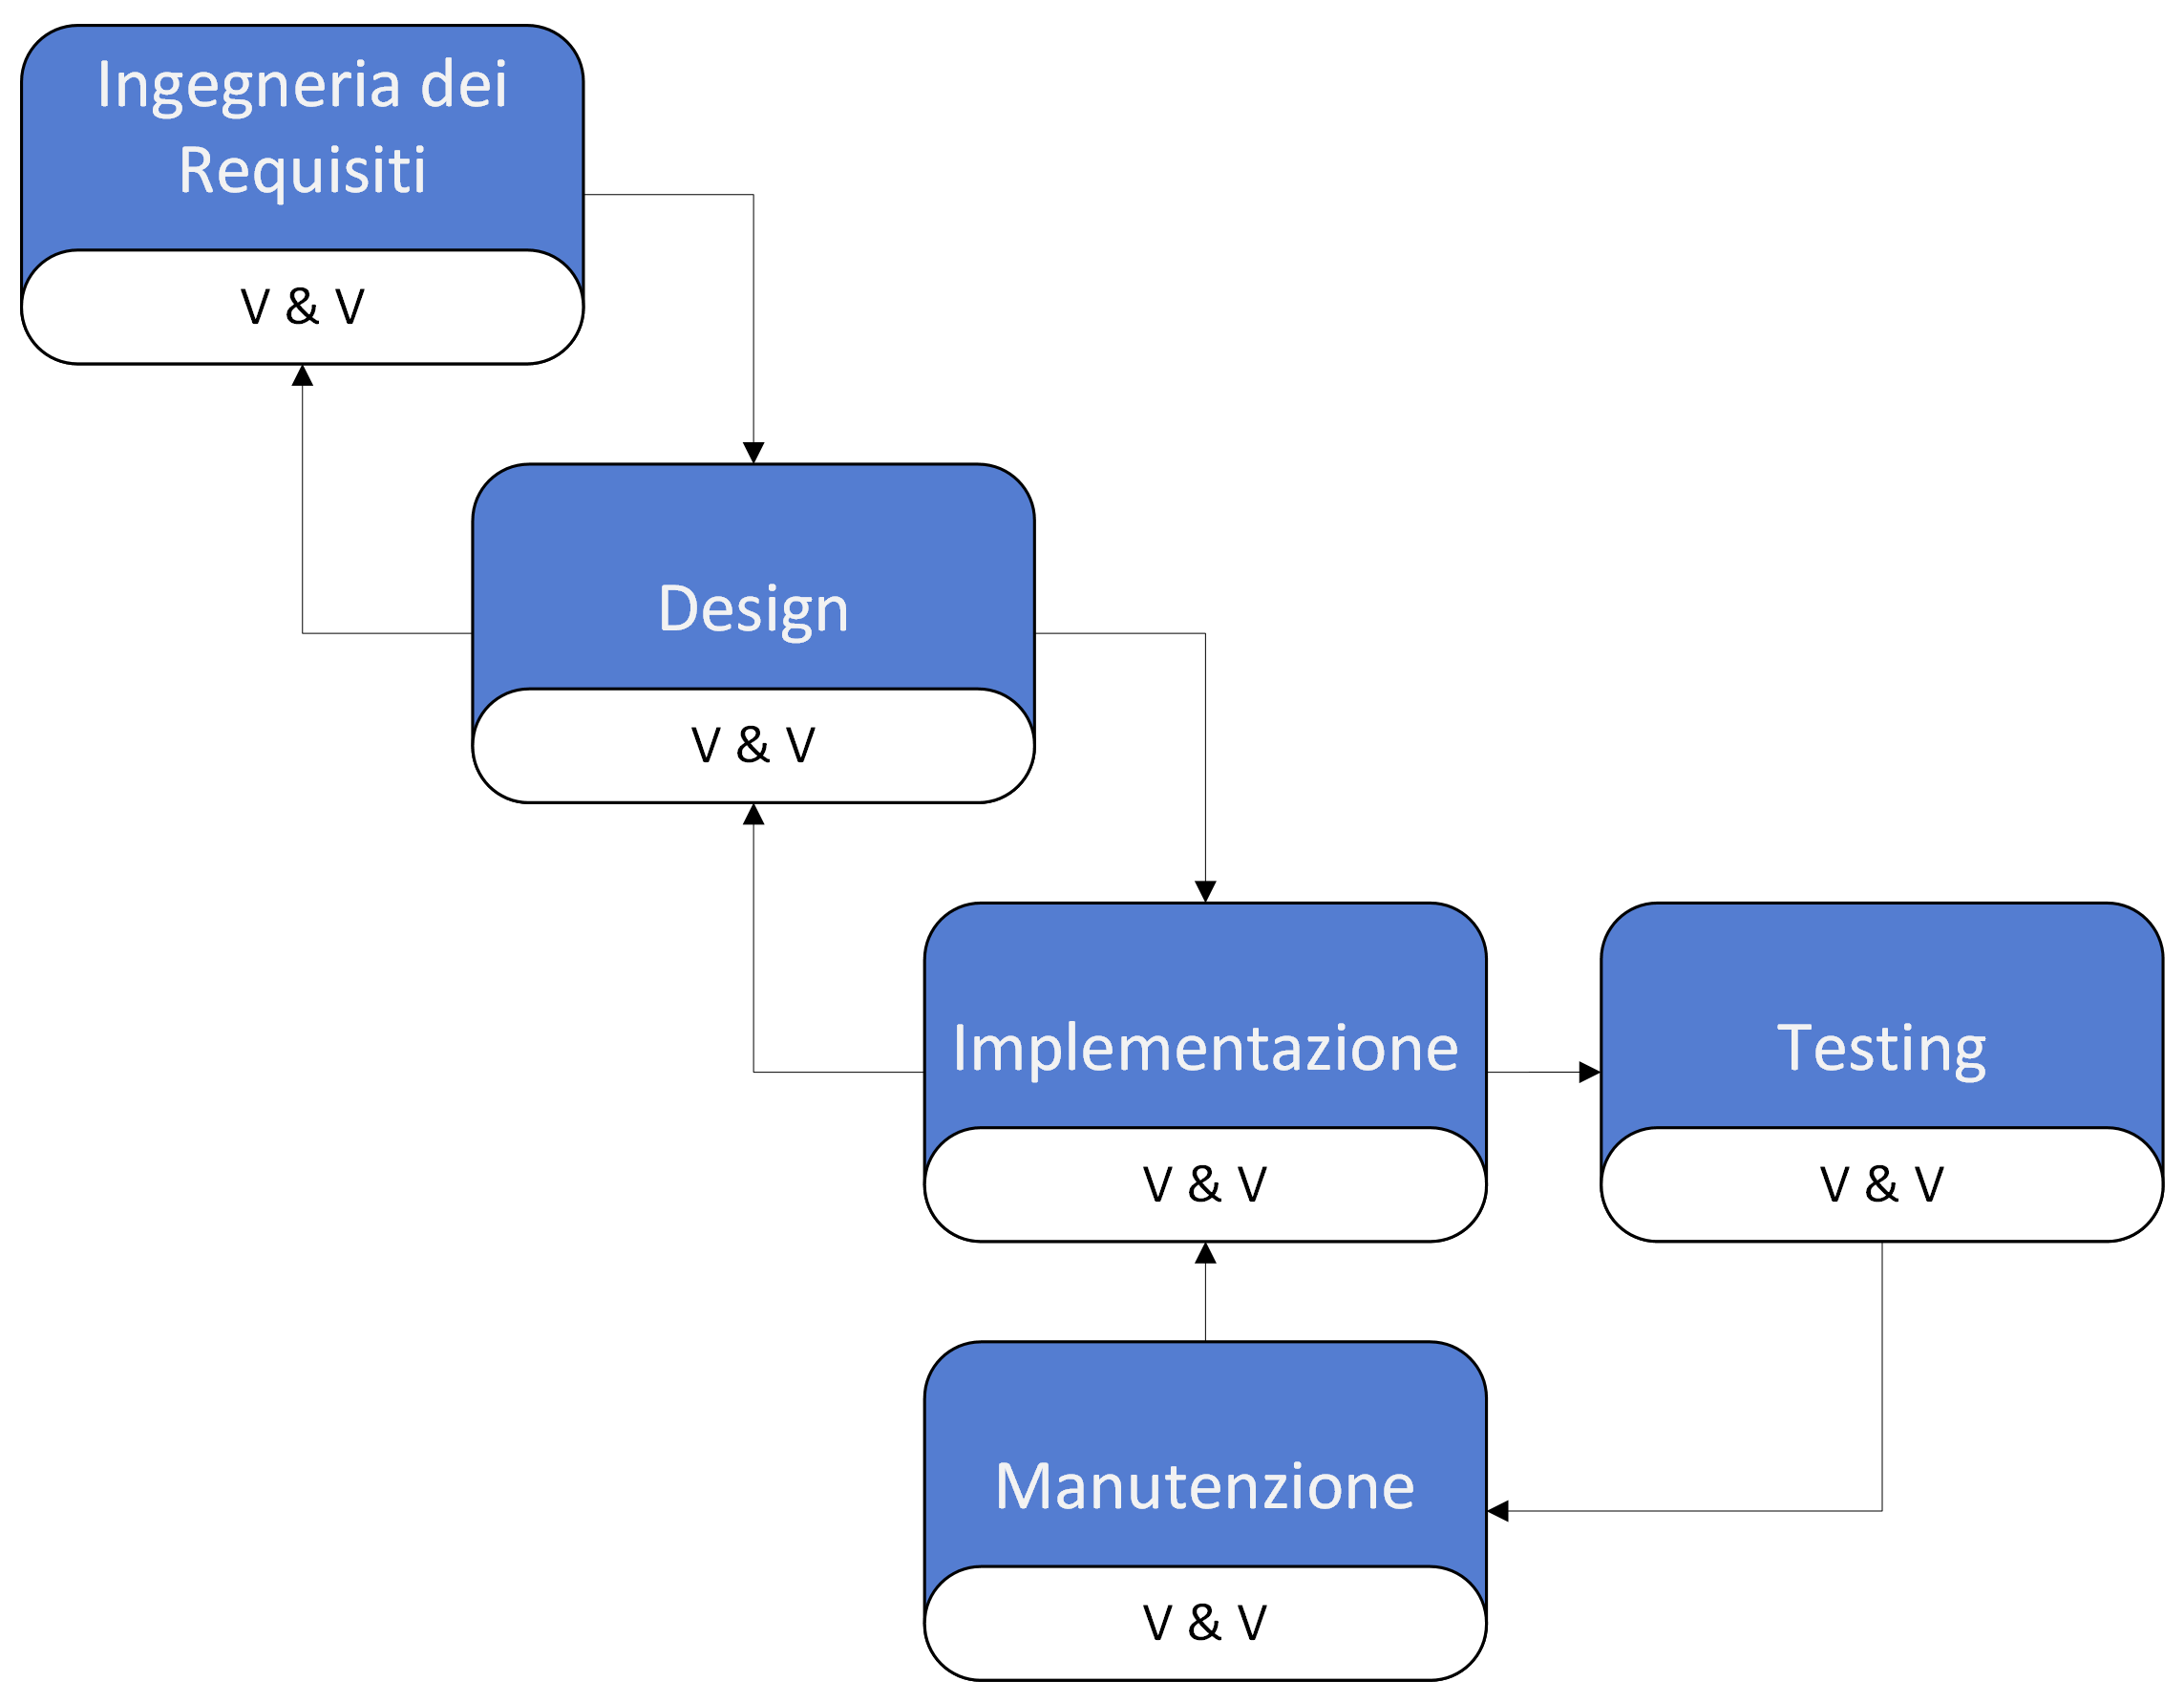
\includegraphics[width=\linewidth]{imgs/Modello a Cascata_0.png}
    \caption{Modello a Cascata Modificato}
    \label{fig:enter-label}
\end{figure}



\subsection{Configuration Management}
\subsubsection{People Management}

\end{document}
